\documentclass{ctexart}
\usepackage{amsmath,bm}
\usepackage{setspace}
\usepackage{xeCJK}
\usepackage{indentfirst}
\usepackage{listings}
\usepackage{graphicx}
\usepackage{subfigure}
\usepackage{amsfonts,amssymb}
\usepackage[a4paper,scale=0.8]{geometry}
\usepackage{hyperref}
\usepackage{pythonhighlight}
\usepackage{float}
\setCJKmainfont{华光书宋_CNKI}
\newCJKfontfamily\kaiti{华光楷体_CNKI}
\newCJKfontfamily\hei{华光黑体_CNKI}
\newCJKfontfamily\fsong{华光仿宋_CNKI}
\newfontfamily\code{Courier New}
\linespread{1.5} \setlength\parindent{2 em}
\title{\Huge 中国科学技术大学计算机学院\\《人工智能基础》实验报告}
\date{\LARGE 2021.07.14}
\begin{document}
\begin{hei}  \maketitle\end{hei}
\begin{figure}[htbp]
    \centering
    
\includegraphics[scale=0.4]{USTC.png}

\end{figure}
\begin{LARGE}\begin{align*} & \text{实验题目:\underline{传统机器学习与深度学习}} \\
         & \text{学生姓名:\underline{胡毅翔}}                 \\
         & \text{学生学号:\underline{PB18000290}}\end{align*}\end{LARGE}
\par
\par\par
\centerline{\large 计算机实验教学中心制}
\par \centerline {\large 2019年9月}
\newpage
\tableofcontents
\newpage
\section{\hei 实验目的}
\begin{enumerate}
    \item 实现线性分类器算法;
    \item 实现朴素贝叶斯分类器;
    \item 实现SVM分类器;
    \item 手写实现感知机模型并进行反向传播;
    \item 实现MLP-Mixer。
\end{enumerate}
\section{\hei 实验环境}
\begin{enumerate}
    \item PC一台;
    \item Windows 10操作系统;
    \item Python 3.8.1;
    \item Pytorch 1.8.1+cpu。
\end{enumerate}

\section{\hei 传统机器学习}
\subsection{\hei 线性分类器算法}
\subsubsection{\hei 最小二乘问题}
\begin{equation}\begin{aligned}
        Loss=\min _{w}(X w-y)^{2}+\lambda\|w\|^{2}                                                                            \\
        \frac{\partial Loss}{\partial w}=2(\mathbf{X} \mathbf{w}-\mathbf{y})^{\top} \mathbf{X}+2\lambda \mathbf{I} w^{\top}=0 \\
        w^{*}= ({\mathbf{X}^{\top}\mathbf{X}+\lambda\mathbf{I})^{\top}}^{-1}\mathbf{X}^{\top}y
    \end{aligned}
\end{equation}
\subsubsection{\hei 算法部分}
基于上述推导的结果,完成的代码如下:
\begin{python}
    '''根据训练数据train_features,train_labels计算梯度更新参数W'''

    def fit(self, train_features, train_labels):
    # 参数weight,bias初始化
    self.weight = np.array(np.random.rand(
    train_features.shape[1], train_labels.shape[1]))
    self.bias = np.zeros(train_labels.shape[1])
    # 计算更新时用的矩阵
    x_T = train_features.transpose()
    a = x_T.dot(train_features)
    a = a + self.Lambda * \
    np.identity(train_features.shape[1], dtype=np.float32)
    a = a.transpose()
    a = np.linalg.inv(a)
    a = a.dot(x_T)
    # 训练 迭代
    for i in range(self.epochs):
    # 预测
    y_pred = self.predict(train_features)
    # 计算梯度
    d_w = a@(y_pred - train_labels)
    d_b = np.mean(y_pred-train_labels)
    # 更新参数
    self.weight = self.weight - self.lr * d_w
    self.bias = self.bias - self.lr * d_b

    '''根据训练好的参数对测试数据test_features进行预测,返回预测结果
    预测结果的数据类型应为np数组,shape=(test_num,1) test_num为测试数据的数目'''

    def predict(self, test_features):
    y_pred_proba = test_features.dot(self.weight)+self.bias
    y_pred = y_pred_proba
    # 预测
    for k in range(y_pred_proba.shape[0]):
    y_pred[k][0] = math.floor(y_pred_proba[k][0])
    return y_pred
\end{python}
\par 运行结果截图如下:
\begin{figure}[htbp]
    \centering
    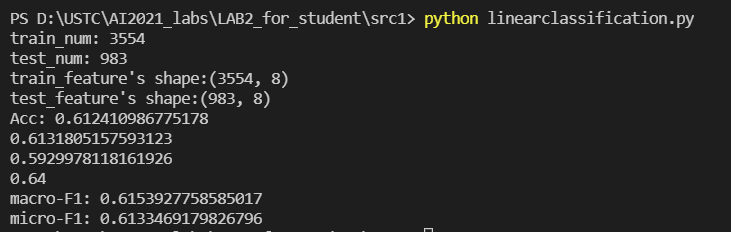
\includegraphics[scale=0.5]{lc.png}

\end{figure}
\subsection{\hei 朴素贝叶斯分类器}
\subsubsection{\hei 实验原理}
\begin{enumerate}
    \item 使用拉普拉斯平滑计算条件概率和先验概率:
          \begin{equation}
              \begin{aligned}
                  \hat{P}(c)                       & =\frac{\left|D_{c}\right|+1}{|D|+N}                           \\
                  \hat{P}\left(x_{i} \mid c\right) & =\frac{\left|D_{c, x_{i}}\right|+1}{\left|D_{c}\right|+N_{i}}
              \end{aligned}
          \end{equation}
          其中 $D$ 表示训练集, $D_{c}$ 表示其中类别为c的数据, $D_{c, x_{i}}$ 表示类别为C,第 $i$ 个属性值为 $x$ 的数据, $N_{i}$ 表示第$i$个属性 可能的取值数。
    \item 判定准则为
          $$
              h_{n\ b}(x)=\operatorname{argmax}_{c \in \mathcal{Y}} P(c) \prod_{i=1}^{d} P\left(x_{i} \mid c\right)
          $$
\end{enumerate}
对于连续变量,假设服从高斯分布,用训练数据估计对应于每个类的均值$\mu$和方差$\sigma^{2}$。
\subsubsection{\hei 算法部分}
基于上述推导的结果,完成的代码如下:
\begin{python}
    '''
    通过训练集计算先验概率分布p(c)和条件概率分布p(x|c)
    建议全部取log,避免相乘为0
    '''

    def fit(self, traindata, trainlabel, featuretype):
    # 计算先验概率
    Py = {}
    yi = {}
    ySet = np.unique(trainlabel)
    for i in ySet:
    # 统计类别为i的数据量
    Py[i] = (sum(trainlabel == i)+1)/(trainlabel.shape[0]+len(ySet))
    yi[i] = sum(trainlabel == i)
    # 保存Pc: P(c) 每个类别c的概率分布
    self.Pc = Py
    ySet = yi
    print("先验概率p(c)计算完毕!")
    # 计算条件概率
    Pxy = {}

    for xIdx in range(len(featuretype)):
    # 第一层不同的属性/特征
    Xarr = traindata[:, xIdx]
    if featuretype[xIdx] == 0:
    # 离散型特征
    categoryParams = {}
    XiSet = np.unique(Xarr)
    XiSetCount = XiSet.size
    for yj, yiCount in ySet.items():
    # 第二层是不同的分类标签
    categoryParams[yj] = {}
    Xiyi = Xarr[np.nonzero(trainlabel == yj)[0]]
    for xi in XiSet:
    # 第三层是变量X的不同值类型
    tmp = (sum(Xiyi == xi)+1)/(Xiyi.size+XiSetCount)
    categoryParams[yj][xi] = tmp
    Pxy[xIdx] = categoryParams
    else:
    # 连续型特征
    continuousParams = {}
    for yk, yiCount in ySet.items():
    # 第二层是不同的分类标签
    Xiyi = Xarr[np.nonzero(trainlabel == yk)[0]]
    continuousParams[yk] = (Xiyi.mean(), Xiyi.std())
    Pxy[xIdx] = continuousParams
    print("条件概率p(x|c)计算完毕!")
    # 保存Pxc: P(c|x) 每个特征的条件概率
    self.Pxc = Pxy
    return

    '''
    根据先验概率分布p(c)和条件概率分布p(x|c)对新样本进行预测
    返回预测结果,预测结果的数据类型应为np数组,shape=(test_num,1) test_num为测试数据的数目
    feature_type为0-1数组,表示特征的数据类型,0表示离散型,1表示连续型
    '''

    def predict(self, features, featuretype):
    m, n = features.shape
    log_proba = np.zeros((m, len(self.Pc)))
    for i in range(m):
    # 第一层每个样本
    for idx, (yi, Py) in enumerate(self.Pc.items()):
    # 第二层不同类别
    # 取对数计算
    log_proba_idx = 0
    for xIdx in range(n):
    # 第三层每种特征
    xi = features[i, xIdx]
    if featuretype[xIdx] == 0:
    log_proba_idx += np.log(self.Pxc[xIdx][yi][xi])
    else:
    miu = self.Pxc[xIdx][yi][0]
    sigma = self.Pxc[xIdx][yi][1]
    t = np.exp(-(xi-miu)**2/(2*sigma**2)) / \
    (np.power(2*np.pi, 0.5)*sigma)
    log_proba_idx += np.log(t)
    log_proba[i, idx] = log_proba_idx+np.log(Py)
    # 选择可能性最大的
    a = np.argmax(log_proba, axis=1)
    a = a + 1
    return a.reshape(m, 1)
\end{python}
\par 运行结果截图如下:
\begin{figure}[htbp]
    \centering
    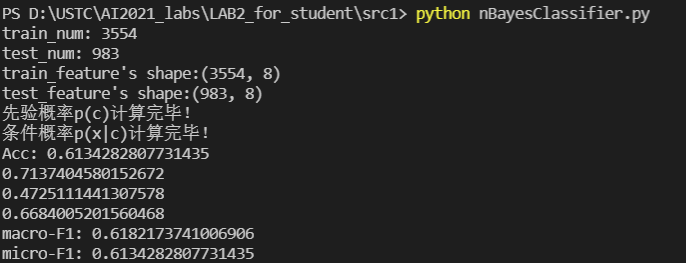
\includegraphics[scale=0.5]{nb.png}

\end{figure}
\subsection{\hei SVM分类器}
\subsubsection{\hei 实验原理}
课堂中所学的SVM分类器用于解决的时二分类问题。本次实验需要解决的是K分类问题。
\par 对于K分类(K>2),我们使用one-vs-all策略训练,具体为:对于任一类别,
我们将其看作正类“1”,其余类别看作负
类“-1”, 分别训练得到K个二分类器;测试时,对于一给定样本,分别计算该样本
在K个二分类器上的输出/分数,取
最大输出/分数所对应的分类器的正类作为最终的预测类别。
\par 因此在预测时,计算的返回值不需要经过sign()函数。
\par 在求解时,需要用到凸优化包cvxopt,求解线性规划问题,调用Cvxopt.solvers.qp(P,q,G,h,A,b),求解的问题格式如下:
\begin{equation}
    \begin{aligned}
         & \operatorname{minimize} \quad(1 / 2) x^{T} P x+q^{T} x \\
         & \text { subject to } G x \preceq h                     \\
         & A x=b
    \end{aligned}
\end{equation}
\par 或
\begin{equation}
    \begin{array}{cl}
        \operatorname{maximize} & -(1 / 2)\left(q+G^{T} z+A^{T} y\right)^{T} P^{\dagger}\left(q+G^{T} z+A^{T} y\right)-h^{T} z-b^{T} y \\
        \text { subject to }    & q+G^{T} z+A^{T} y \in \operatorname{range}(P)                                                        \\
                                & z \succeq 0
    \end{array}
\end{equation}
\par 例如:
\begin{equation}
    \begin{array}{ll}
        \min                 & 2 x_{1}^{2}+x_{2}^{2}+x_{1} x_{2}+x_{1}+x_{2} \\
        \text { s.t. } \quad & x_{1} \geq 0                                  \\
                             & x_{2} \geq 0                                  \\
                             & x_{1}+x_{2}=1
    \end{array}
\end{equation}
\par 或
\begin{equation}
    \begin{array}{ll}
        \min                 & 2 x_{1}^{2}+x_{2}^{2}+x_{1} x_{2}+x_{1}+x_{2} \\
        \text { s.t. } \quad & -x_{1} \leq 0                                 \\
        \quad                & -x_{2} \leq 0                                 \\
                             & x_{1}+x_{2}=1
    \end{array}
\end{equation}
\subsubsection{\hei 算法部分}
基于上述推导的结果,完成的代码如下:
\begin{python}
    def fit(self, train_data, train_label, test_data):
    # 构造核矩阵K,Kij = <yixi,yjxj>
    train_num = train_data.shape[0]
    K = np.zeros((train_num, train_num))
    temp = train_data
    for i in range(train_num):
    for j in range(train_num):
    K[i][j] = self.KERNEL(
    temp[i], temp[j], self.kernel)*train_label[i]*train_label[j]

    # 构造q
    q = np.ones((train_num, 1))
    q = -1*q
    # 构造G
    G1 = np.eye(train_num, dtype=int)
    G2 = np.eye(train_num, dtype=int)
    G2 = -1*G2
    G = np.r_[G1, G2]
    # 构造h
    h1 = np.zeros((train_num, 1))
    for i in range(train_num):
    h1[i] = self.C
    h2 = np.zeros((train_num, 1))
    h = np.r_[h1, h2]
    # 构造A
    A = train_label.reshape(1, train_num)
    # 构造b
    b = np.zeros((1, 1))
    # 统一数据类型
    K = K.astype(np.double)
    q = q.astype(np.double)
    G = G.astype(np.double)
    h = h.astype(np.double)
    A = A.astype(np.double)
    b = b.astype(np.double)
    # 化成cvxopt.matrix格式
    K_1 = cvxopt.matrix(K)
    q_1 = cvxopt.matrix(q)
    G_1 = cvxopt.matrix(G)
    h_1 = cvxopt.matrix(h)
    A_1 = cvxopt.matrix(A)
    b_1 = cvxopt.matrix(b)
    # 用cvxopt(凸优化包)求解约束方程
    sol = cvxopt.solvers.qp(K_1, q_1, G_1, h_1, A_1, b_1)
    sol_x = sol['x']
    alpha = np.array(sol_x)
    indices = np.where(alpha > self.Epsilon)[0]
    bias = np.mean(
    [train_label[i] - sum([train_label[i] * alpha[i] * self.KERNEL(x, train_data[i], self.kernel) for x in train_data[indices]]) for i in indices])
    test_num = test_data.shape[0]
    # 预测
    predictions = []
    for j in range(test_num):
    prediction = bias + sum([train_label[i] * alpha[i] * self.KERNEL(
    test_data[j], train_data[i], self.kernel) for i in indices])
    predictions.append(prediction)
    prediction = np.array(predictions).reshape(test_num, 1)
    return prediction
\end{python}
\par 核函数类型为Linear时,运行结果截图如下:
\begin{figure}[htbp]
    \centering
    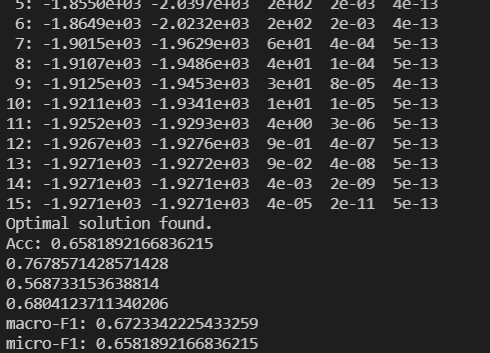
\includegraphics[scale=0.5]{linear1.png}

\end{figure}
\par 核函数类型为Poly时,运行结果截图如下:
\begin{figure}[H]
    \centering
    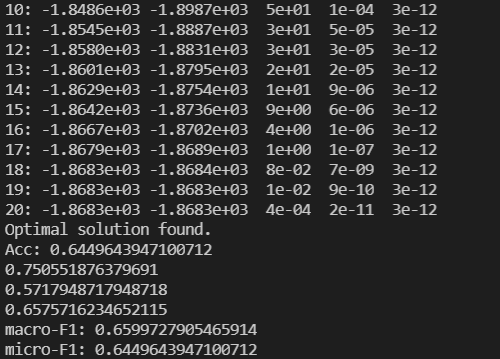
\includegraphics[scale=0.5]{Ploy.png}

\end{figure}
\par 核函数类型为Gauss时,运行结果截图如下:
\begin{figure}[H]
    \centering
    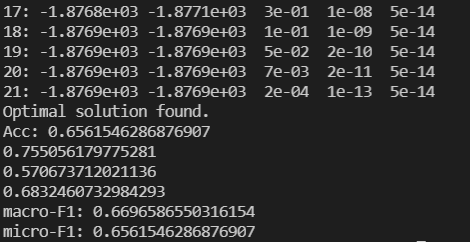
\includegraphics[scale=0.5]{gauss.png}

\end{figure}
\section{\hei 深度学习}
\subsection{\hei 感知机模型}
\subsubsection{\hei 实验原理}
多层感知机由感知机推广而来,最主要的特点是有多个神经元层,因此也叫深度神经网络(DNN: Deep Neural Networks)。
\par 多层感知机的一个重要特点就是多层,我们将第一层称之为输入层,最后一层称之有输出层,中间的层称之为隐层。
MLP并没有规定隐层的数量,因此可以根据各自的需求选择合适的隐层层数。且对于输出层神经元的个数也没有限制。
\par 首先进行MLP梯度推导。
\par 单输出感知器模型的运算法则:
\begin{equation}
    \begin{aligned}
         & y=X W+b                \\
         & y=\sum x_{i} * w_{i}+b
    \end{aligned}
\end{equation}
\par 输入X乘以权重W得到y,再通过激活函数得到输出(O)。在这里,激活函数是sigmoid函数。
\begin{equation}
    \sigma(y)=\frac{1}{1+e^{-y}}
\end{equation}
\par E是loss函数值,这里是输出值(output)与真实值(target)的欧式距离。
\begin{equation}
    E=\frac{1}{2}\left(O_{0}^{1}-t\right)^{2}
\end{equation}
\par E的大小是评价感知器模型好坏的指标之一,w权重是描述这个感知器模型的参数,通过计算E来优化感知器模型,即优化w的值。$w_{j k}^{I}$
表示第I层,第j个输入链接第k个输出的权值w。以下先对一个权重(值)w求得感知器模型的梯度。
\begin{equation}
    \begin{aligned}
        \frac{\partial E}{\partial w_{j 0}^{1}} & =\left(O_{0}^{1}-t\right) \frac{\partial O_{0}^{1}}{\partial w_{j 0}^{1}}                                                                  \\
        \frac{\partial E}{\partial w_{j 0}^{1}} & =\left(O_{0}^{1}-t\right) \frac{\partial \sigma\left(x_{0}^{1}\right)}{\partial w_{j 0}^{i}}                                               \\
        \frac{\partial E}{\partial w_{j 0}^{1}} & =\left(O_{0}^{1}-t\right) \frac{\partial \sigma\left(x_{0}^{1}\right)}{\partial x_{0}^{1}} \frac{\partial x_{0}^{1}}{\partial w_{j 0}^{1}}
    \end{aligned}
\end{equation}
\par 红色部分使用了链式法则,链式法则其实就是连续求导,这里将求得sigmoid函数的导数。sigmoid导数如何求,将在下一环节展示。求得的sigmoid导数是$s\prime(x) = s(x)(1 - s(x))$。
\begin{equation}
    \begin{aligned}
        \frac{\partial E}{\partial w_{j 0}^{1}} & =\left(O_{0}^{1}-t\right) \sigma\left(x_{0}^{1}\right)\left(1-\sigma\left(x_{0}^{1}\right)\right) \frac{\partial x_{0}^{1}}{\partial w_{j 0}^{1}} \\
        \frac{\partial E}{\partial w_{j 0}^{1}} & =\left(O_{0}^{1}-t\right) O_{0}^{1}\left(1-O_{0}^{1}\right) \frac{\partial x_{0}^{1}}{\partial w_{j 0}^{1}}                                       \\
        \frac{\partial E}{\partial w_{j 0}^{1}} & =\left(O_{0}^{1}-t\right) O_{0}^{1}\left(1-O_{0}^{1}\right) x_{j}^{0}
    \end{aligned}
\end{equation}
\par 现在把单个输出的感知器模型推广成多输出感知器模型。按照上面的思路,求w的梯度:
\begin{equation}
    \begin{aligned}
         & E=\frac{1}{2} \sum\left(O_{i}^{1}-t_{i}\right)^{2}                                                                    \\
         & \frac{\partial E}{\partial u_{j k}^{1}}=\left(O_{k}^{1}-t_{k}\right) \frac{\partial Q_{ k}^{1}}{\partial w_{j k}^{1}}
    \end{aligned}
\end{equation}
\par $W_{j k}$只对$O_{k}$值有贡献,对$O_{i}$(i不等于k)没有贡献。因此$O_{i}$(i不等于k)对$W_{j k}$的偏导为0。换句话说,相关梯度与输入结点有关。
\begin{equation}
    \begin{aligned}
        \frac{\partial E}{\partial w_{j k}^{1}} & =\left(O_{k}^{1}-t_{k}\right) \frac{\partial \sigma\left(x_{k}^{1}\right)}{\partial w_{j k}^{1}}                                                             \\
        \frac{\partial E}{\partial w_{j k}^{1}} & =\left(O_{k}^{1}-t_{k}\right) \sigma\left(x_{k}^{1}\right)\left(1-\sigma\left(x_{k}^{1}\right)\right) \frac{\partial x_{k}^{1}}{\partial w_{j k}^{1}} \\
        \frac{\partial E}{\partial w_{j k}^{1}} & =\left(O_{k}^{1}-t_{k}\right) O_{k}^{1}\left(1-O_{k}^{1}\right) x_{j}^{0}
    \end{aligned}
\end{equation}
\par 下面推导MLP链式法则。
\par 求导过程:
\begin{equation}
    \begin{aligned}
    &\left(\frac{f}{g}\right)^{\prime}=\frac{f^{\prime} g-f g^{\prime}}{g^{2}} \\
    &\sigma(y)=\frac{1}{1+e^{-y}} \\
    &\frac{\partial \sigma(y)}{\partial y}=\frac{0 *\left(1+e^{-y}\right)-1 *\left(-e^{-y}\right)}{1+2 e^{-y}+e^{-2 y}} \\
    &=\frac{e^{-y}}{\left(1+e^{-y}\right)^{2}}=\frac{1+e^{-y}-1}{\left(1+e^{-y}\right)^{2}}=\frac{1}{1+e^{-y}}-\frac{1}{\left(1+e^{-y}\right)^{2}} \\
    &=\frac{1}{1+e^{-y}}\left(1-\frac{1}{1+e^{-y}}\right)=\sigma(y)(1-\sigma(y))
    \end{aligned}
    \end{equation}
\par 链式法则如下:
\begin{equation}
    \frac{\partial E}{\partial w_{j k}^{1}}=\frac{\partial E}{\partial O_{k}^{1}} \frac{\partial O_{k}^{1}}{\partial w_{j k}^{1}}=\frac{\partial E}{\partial O_{k}^{2}} \frac{\partial O_{k}^{2}}{\partial O_{k}^{1}} \frac{\partial O_{k}^{1}}{\partial w_{j k}^{1}}
\end{equation}
\par 最后推导MLP反向传播。
\par 参考上面的公式推导,现在完成从1到K的泛化处理。首先根据前面的结论,梯度推导为:
\begin{equation}
    \frac{\partial E}{\partial w_{j k}^{K}}=\left(O_{k}^{K}-t_{k}\right) O_{k}^{K}\left(1-O_{k}^{K}\right) x_{j}^{K-1}
    \end{equation}
\par 针对多层感知器,x是该层的输入,即是上一层的输出O。如果这里用x表示会有歧义,因为O = sigmoid(x),x必须经过激活函数之后才会得到O,所以对多层感知器而言,梯度推导为:
\begin{equation}
    \frac{\partial E}{\partial w_{j k}^{K}}=\left(O_{k}^{K}-t_{k}\right) O_{k}^{K}\left(1-O_{k}^{K}\right) O_{j}^{K-1}
    \end{equation}
\par 现在,我们对结合上述结论,以及链式法则,完成下一层的梯度求导,即对$w_{i j}^{J}$求导。
\begin{equation}
    \begin{aligned}
    \frac{\partial E}{\partial w_{i j}^{J}} &=\frac{\partial}{\partial w_{i j}^{J}} \frac{1}{2} \sum_{k \in K}\left(O_{k}^{K}-t_{k}\right)^{2} \\
    \frac{\partial E}{\partial w_{i j}^{J}} &=\sum_{k \in K}\left(O_{k}^{K}-t_{k}\right) \frac{\partial}{\partial w_{i j}^{J}} O_{k}^{K} \\
    \frac{\partial E}{\partial w_{i j}^{J}} &=\sum_{k \in K}\left(O_{k}^{K}-t_{k}\right) \frac{\partial}{\partial w_{i j}^{J}} \sigma\left(x_{k}^{K}\right) \\
    \frac{\partial E}{\partial w_{i j}^{J}} &=\sum_{k \in K}\left(O_{k}^{K}-t_{k}\right) \frac{\partial \sigma\left(x_{k}^{K}\right)}{\partial x_{k}^{K}} \frac{\partial x_{k}^{K}}{\partial w_{i j}^{J}} \\
    \frac{\partial E}{\partial w_{i j}^{J}} &=\sum_{k \in K}\left(O_{k}^{K}-t_{k}\right) \sigma\left(x_{k}^{K}\right)\left(1-\sigma\left(x_{k}^{K}\right)\right) \frac{\partial x_{k}^{K}}{\partial w_{i j}^{J}}
    \end{aligned}
    \end{equation}
\par 先求到K层的梯度,继续使用链式法则,在K层的梯度上继续求第J层。
\begin{equation}
    \begin{aligned}
    \frac{\partial E}{\partial w_{i j}^{J}} &=\sum_{k \in K}\left(O_{k}^{K}-t_{k}\right) O_{k}^{K}\left(1-O_{k}^{K}\right) \mid \frac{\partial x_{k}^{K}}{\partial O_{j}^{J}} \frac{\partial O_{j}^{j}}{\partial w_{i j}^{J}} \\
    \frac{\partial E}{\partial w_{i j}^{J}} &=\sum_{k \in K}\left(O_{k}^{K}-t_{k}\right) O_{k}^{K}\left(1-O_{k}^{K}\right) \sqrt{w_{j k}^{K}}{\partial \frac{\partial O_{j}^{J}}{\partial w_{i j}^{J}}} \\
    \frac{\partial E}{\partial w_{i j}^{J}} &=\frac{\partial O_{j}^{J}}{\partial w_{i j}^{J}} \sum_{k \in K}\left(O_{k}^{K}-t_{k}\right) O_{k}^{K}\left(1-O_{k}^{K}\right) w_{j k}^{K} \\
    \frac{\partial E}{\partial w_{i j}^{J}} &=\frac{\partial \sigma\left(x_{j}^{J}\right)}{\partial x_{j}^{J}} \frac{\partial x_{j}^{J}}{\partial w_{i j}^{J}} \sum_{k \in K}\left(O_{k}^{K}-t_{k}\right) O_{k}^{K}\left(1-O_{k}^{K}\right) w_{j k}^{K} \\
    \frac{\partial E}{\partial w_{i j}^{J}} &=O_{j}^{J}\left(1-O_{j}^{J}\right) \frac{\partial x_{j}^{J}}{\partial w_{i j}^{J}} \sum_{k \in K}\left(O_{k}^{K}-t_{k}\right) O_{k}^{K}\left(1-O_{k}^{K}\right) w_{j k}^{K} \\
    \frac{\partial E}{\partial w_{i j}^{J}} &=O_{j}^{J}\left(1-O_{j}^{J}\right) O_{i}^{I} \sum_{k \in K}\left(O_{k}^{K}-t_{k}\right) O_{k}^{K}\left(1-O_{k}^{K}\right) w_{j k}^{K}
    \end{aligned}
    \end{equation}
\par I,J,K是连续的3层,即J = I + 1,K = J + 1。现在开始对其简化。对第K层的第k结点有:
\begin{equation}
    \frac{\partial E}{\partial w_{j k}^{K}}=O_{j}^{J} \delta_{k}^{K}
    \end{equation}
\par 其中:
\begin{equation}
    \delta_{k}^{K}=\left(O_{k}^{K}-t_{k}\right) O_{k}^{K}\left(1-O_{k}^{K}\right)
    \end{equation}
\par 同理,对第J(K = J + 1)层的第j个结点有:
\begin{equation}
    \frac{\partial E}{\partial w_{i j}^{J}}=O_{i}^{l} \delta_{j}^{J}
    \end{equation}
\par 其中:
\begin{equation}
    \delta_{j}^{J}=O_{j}^{J}\left(1-O_{j}^{J}\right) \sum_{k \in K} \delta_{k}^{K}  w_{j k}^{K}
    \end{equation}
    现在开始说反向传播。如果通过前向通路求得个个参数的梯度十分困难和繁琐。比如需要先对第I层求得梯度,然后又求得第J层,最后是第K层。这样会重复计算,会造成资源浪费。
    如果使用反向传播的话,可以一次计算所有参数。如同上述推导过程一样,如果要对第J层(第J层不是输出层,第K层是输出层)求得梯度,那么必须要经过求得第K层(输出层)梯度基础上才行,第I层,I-1,...,0层(输入层)同理。
\subsubsection{\hei 算法部分}
代码详见MLP\_manual.py。
\par 运行结果截图如下:
\begin{figure}[htbp]
    \centering
    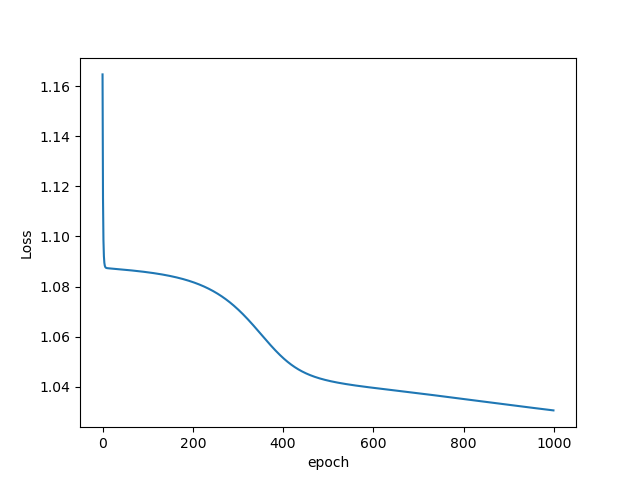
\includegraphics[scale=0.5]{Figure_1.png}

\end{figure}
\subsection{\hei MLPMixer}
\subsubsection{\hei 实验原理}
MLP-Mixer主要包括三部分:Per-patch Fully-connected、Mixer Layer、分类器。其中分类器部分采用传统的
全局平均池化(GAP)+全连接层(FC)+Softmax的方式构成,故不进行更多介绍,下面主要针对前两部分进行解释。
\par 首先介绍全连接部分。
\par FC相较于Conv,并不能获取局部区域间的信息,为了解决这个问题,MLP-Mixer通过Per-patch Fully-connected将输入图像转化为2D的Table,方便在后面进行局部区域间的信息融合。
\par 具体来说,MLP-Mixer将输入图像相邻无重叠地划分为S个Patch,每个Patch通过MLP映射为一维特征向量,其中一维向量长度为C,最后将每个Patch得到的特征向量组合得到大小为S*C的2D Table。需要注意的时,每个Patch使用的映射矩阵相同,即使用的MLP参数相同。
\par 实际上,Per-patch Fully-connected实现了(W,H,C)的向量空间到(S,C)的向量空间的映射。
\par 例如,假设输入图像大小为240*240*3,模型选取的Patch为16*16,那么一张图片可以划分为(240*240)/(16*16)= 225个Patch。结合图片的通道数,每个Patch包含了16*16*3 = 768个值,把这768个值做Flatten作为MLP的输入,其中MLP的输出层神经元个数为128。这样,每个Patch就可以得到长度的128的特征向量,组合得到225*128的Table。MLP-Mixer中Patch大小和MLP输出单元个数为超参数。
\par 再介绍Mixer Layer部分。
\par 观察Per-patch Fully-connected得到的Table会发现,Table的行代表了同一空间位置在不同通道上的信息,列代表了不同空间位置在同一通道上的信息。换句话说,对Table的每一行进行操作可以实现通道域的信息融合,对Table的每一列进行操作可以实现空间域的信息融合。
\par 在传统CNN中,可以通过1*1 Conv来实现通道域的信息融合,如果使用更大一点的卷积核,可以同时实现空间域和通道域的信息融合。

\par 在Transformer中,通过Self-Attention实现空间域的信息融合,通过MLP同时实现空间域和通道域的信息融合。

\par 而在MLP-Mixer中,通过Mixer Layer使用MLP先后对列、行进行映射,实现空间域和通道域的信息融合。与传统卷积不同的是,Mixer Layer将空间域和通道域分开操作,这种思想与Xception和MobileNet中的深度可分离卷积相似。
\begin{figure}[htbp]
    \centering
    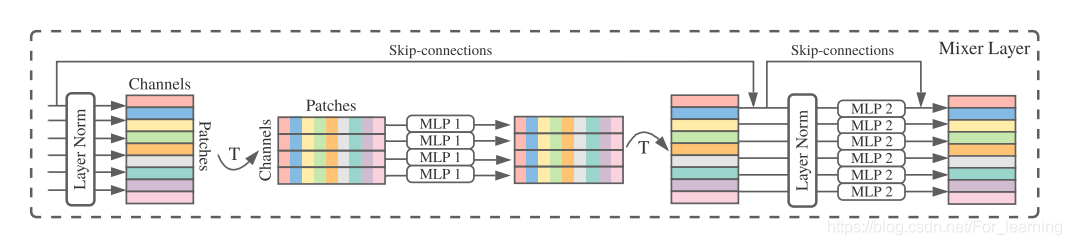
\includegraphics[scale=0.5]{mix1.png}

\end{figure}
\par 根据上述内容,MLP-Mixer在Mixer Layer中使用分别使用token-mixing MLPs(图中MLP1)和channel-mixing MLPs(图中MLP2)对Table的列和行进行映射,与Per-patch Fully-connected相同,MLP1和MLP2在不同列、行中的映射过程中共享权重。除此之外,Mixer Layer还加入了LN和跳接来提高模型性能。

\par 另外,MLP1和MLP2都采用了相同的结构,如下图。
\begin{figure}[H]
    \centering
    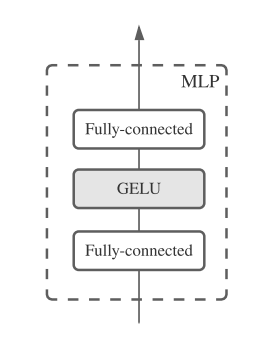
\includegraphics[scale=0.5]{mix2.png}

\end{figure}
\par 整体结构如下:
\begin{figure}[H]
    \centering
    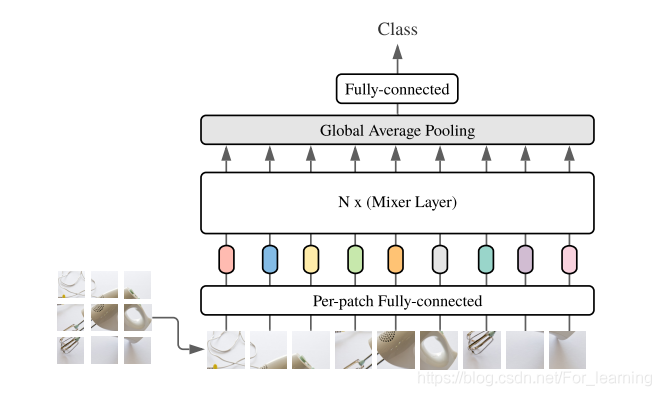
\includegraphics[scale=0.5]{mix3.png}

\end{figure}
\subsubsection{\hei 算法部分}
基于上述原理,完成的代码如下:
\begin{python}
class MLP(nn.Module):
    def __init__(self, dims, multiplxer=4):
        super(MLP, self).__init__()
        hidden = int(dims * multiplxer)

        self.out = nn.Sequential(
            nn.Linear(dims, hidden),
            nn.GELU(),
            nn.Linear(hidden, dims)
        )

    def forward(self, x):
        return self.out(x)


class MixerLayer(nn.Module):
    def __init__(self, patch_size, hidden_dim):
        super(MixerLayer, self).__init__()
        seq = patch_size
        dims = hidden_dim
        # LayerNorm1
        self.layer_norm1 = nn.LayerNorm(dims)
        # mlp1
        self.mlp1 = MLP(seq, multiplxer=0.5)
        # LayerNorm2
        self.layer_norm2 = nn.LayerNorm(dims)
        # mlp2
        self.mlp2 = MLP(dims)

    def forward(self, x):
        out = self.layer_norm1(x).transpose(1, 2)
        out = self.mlp1(out).transpose(1, 2)
        out += x
        out2 = self.layer_norm2(out)
        out2 = self.mlp2(out2)
        out2 += out
        return out2


class MLPMixer(nn.Module):
    def __init__(self, patch_size, hidden_dim, depth):
        super(MLPMixer, self).__init__()
        assert 28 % patch_size == 0, 'image_size must be divisible by patch_size'
        assert depth > 1, 'depth must be larger than 1'
        # 图片大小
        in_dims = 28
        # 维度
        dims = hidden_dim
        # 深度
        N = depth
        # 目标类别数
        n_classes = 10
        self.embedding = nn.Linear(in_dims, dims)
        self.layers = nn.ModuleList()
        for _ in range(N):
            self.layers.append(MixerLayer(in_dims, dims))
        self.gap = nn.AdaptiveAvgPool1d(1)
        self.fc = nn.Linear(dims, n_classes)
        self.dims = dims

    def forward(self, x):
        out = self.embedding(x)
        out = out.permute(0, 2, 3, 1).view(x.size(0), -1, self.dims)
        for layer in self.layers:
            out = layer(out)
        out = out.mean(dim=1)
        out = self.fc(out)
        return out
# 定义训练函数


def train(model, train_loader, optimizer, n_epochs, criterion):
    model.train()
    for epoch in range(n_epochs):
        for batch_idx, (data, target) in enumerate(train_loader):
            batch_size_train = data.shape[0]
            data, target = data.to(device), target.to(device)
            optimizer.zero_grad()
            pre_out = model(data)
            targ_out = torch.nn.functional.one_hot(target, num_classes=10)
            targ_out = targ_out.view((batch_size_train, 10)).float()
            loss = criterion(pre_out, targ_out)
            loss.backward()
            optimizer.step()
            if batch_idx % 100 == 0:
                print('Train Epoch: {}/{} [{}/{}]\tLoss: {:.6f}'.format(
                    epoch, n_epochs, batch_idx * len(data), len(train_loader.dataset), loss.item()))

# 定义测试函数


def test(model, test_loader, criterion):
    model.eval()
    test_loss = 0
    num_correct = 0
    total = 0
    with torch.no_grad():
        for data, target in test_loader:
            batch_size_test = data.shape[0]
            data, target = data.to(device), target.to(device)
            pre_out = model(data)
            targ_out = torch.nn.functional.one_hot(target, num_classes=10)
            targ_out = targ_out.view((batch_size_test, 10)).float()
            test_loss += criterion(pre_out, targ_out)  # 将一批的损失相加
            t = pre_out.argmax(dim=1)
            num_correct += sum(t == target)
            total += batch_size_test
    # 准确率
    accuracy = num_correct/total
    # 平均损失
    test_loss /= len(test_loader.dataset)
    print("Test set: Average loss: {:.4f}\t Acc {:.2f}".format(
        test_loss, accuracy))


if __name__ == '__main__':
    n_epochs = 5
    batch_size = 128
    learning_rate = 0.001

    transform = transforms.Compose(
        [transforms.ToTensor(),
         transforms.Normalize((0.1307,), (0.3081,))])

    trainset = MNIST(root='./data', train=True,
                     download=True, transform=transform)
    train_loader = torch.utils.data.DataLoader(
        trainset, batch_size=batch_size, shuffle=True, num_workers=2)

    testset = MNIST(root='./data', train=False,
                    download=True, transform=transform)
    test_loader = torch.utils.data.DataLoader(
        testset, batch_size=batch_size, shuffle=False, num_workers=2)

    # device = torch.device("cpu")
    device = torch.device("cuda:0" if torch.cuda.is_available() else "cpu")

    #n = (28 * 28) // 4 ** 2
    model = MLPMixer(patch_size=4, hidden_dim=14, depth=12)
    model.to(device)

    optimizer = torch.optim.Adam(model.parameters(), lr=learning_rate)

    mse = nn.MSELoss()

    train(model, train_loader, optimizer, n_epochs, mse)

    test(model, test_loader, mse)
\end{python}
\par 运行结果截图如下:
\begin{figure}[H]
    \centering
    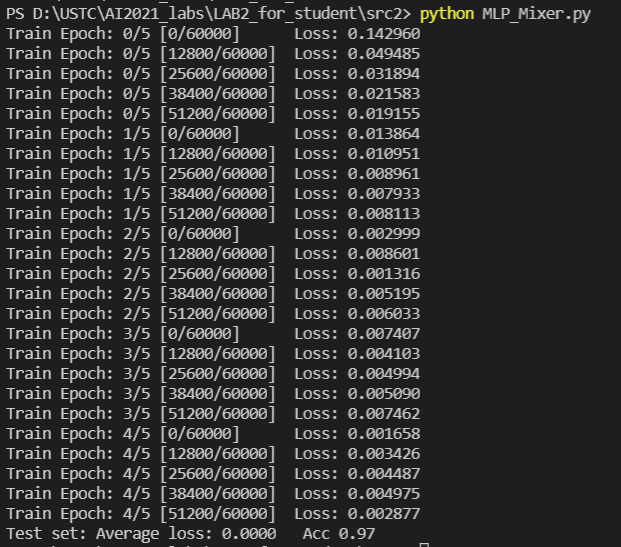
\includegraphics[scale=0.5]{MLPMixer.png}

\end{figure}
\end{document}